% !TeX encoding = utf8
% !TeX program = xelatex
% !BIB program = bibtex
%
% Configuration options:
% english - Use for English language theses
% german - Use for German language theses
% ba - Use for Bachelor theses
% ma - Use for Master theses
\documentclass[english,ba]{tudo-sse-thesis}

% Add the packages necessary
\usepackage[math]{blindtext}
\usepackage{graphicx}

% Provide your title
\title{Diffusion-based Inpainting for Removing Traffic Signals from Distributed Acoustic Sensing Data}

% Provide your name
\author{Islem Dhouioui}

% Provide examiner names. First examiner has a reasonable default and only needs to changed if the default does not fit.
% \firstexaminer{JProf.\ Dr.-Ing.\ Ben Hermann} % Default value
\firstexaminer{Prof.\ Dr.\ Stefan Harmeling}
% \secondexaminer{Prof.\ Dr.\ Zweiter Gutachter}
\secondexaminer{Sebastian Konietzny, M.Sc.}

\begin{document}

\maketitle

\pagenumbering{roman}

% Only add for english documents
\begin{abstract}

Distributed Acoustic Sensing (DAS) enables the measurement of vibrations
along optical fibres with high spatial resolution. In seismic monitoring,
DAS recordings may contain earthquake signals together with
traffic-induced disturbances, which can make the interpretation of the
data more difficult. This thesis investigates diffusion-based inpainting
methods for removing traffic-related structures from DAS data while
preserving relevant seismic information.

A diffusion model is trained on traffic-free DAS patches containing
background noise and earthquake signals. The learned model is then used
as a generative prior to reconstruct masked traffic regions. Different
network architectures for modelling long-range structures are investigated,
together with RePaint and Region-Aware Diffusion (RAD) for the inpainting
process. In addition, traffic-mask generation is considered in order to
separate traffic-related structures from earthquake signals before
reconstruction.

The aim of the work is to develop a DAS-specific inpainting approach that
can suppress traffic disturbances while maintaining the underlying
earthquake-related signal structures.

\end{abstract}

% This needs to be in German or English documents
\begin{abstract-ger}

Distributed Acoustic Sensing (DAS) ermöglicht die räumlich hochaufgelöste
Messung von Vibrationen entlang optischer Fasern. Bei seismischen
Messungen können Erdbebensignale gemeinsam mit verkehrsbedingten
Störungen auftreten und dadurch die Interpretation der Daten erschweren.
Diese Arbeit untersucht diffusionsbasierte Inpainting-Verfahren zur
Entfernung verkehrsbedingter Strukturen aus DAS-Daten unter Erhaltung
relevanter seismischer Informationen.

Dazu wird ein Diffusionsmodell auf verkehrsfreien DAS-Ausschnitten
trainiert, die Hintergrundrauschen und Erdbebensignale enthalten.
Das gelernte Modell wird anschließend als generatives Prior zur
Rekonstruktion maskierter Verkehrsbereiche verwendet. Zusätzlich werden
verschiedene Netzwerkarchitekturen zur Modellierung weitreichender
Strukturen sowie RePaint und Region-Aware Diffusion (RAD) für den
Inpainting-Prozess untersucht.

Ziel der Arbeit ist die Entwicklung eines DAS-spezifischen
Inpainting-Verfahrens, das verkehrsbedingte Störungen unter möglichst
weitgehender Erhaltung der zugrunde liegenden Erdbebenstrukturen
reduziert.

\end{abstract-ger}

\tableofcontents
\cleardoublepage

\pagenumbering{arabic}

% Add your content here

\chapter{Introduction}

\section{Motivation}

Distributed Acoustic Sensing (DAS) is a sensing technology that uses
optical fibres to measure vibrations along the length of a cable.
Laser pulses are transmitted through the fibre, and disturbances caused
by vibrations affect the backscattered light. This allows a single
optical fibre to act as a large number of spatially distributed sensing
points. DAS measurements can therefore provide information over long
distances with a high spatial resolution.
\begin{figure}[htbp]
    \centering
    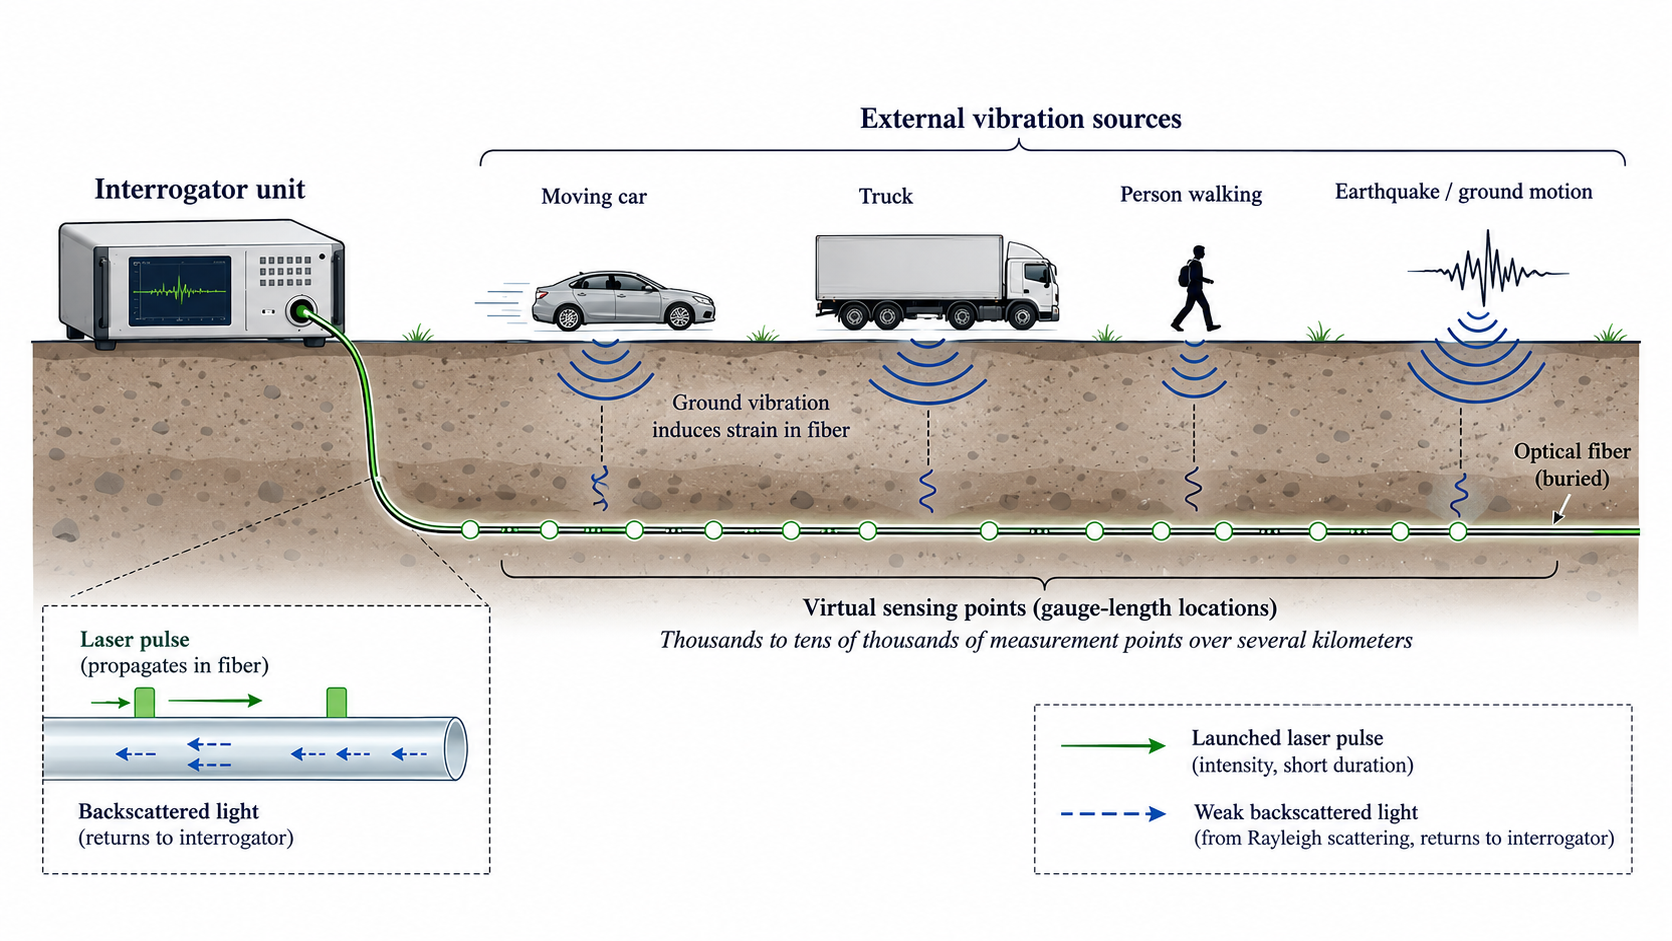
\includegraphics[width=0.78\linewidth]{DAS-Faserdiagramm.png}
    \caption{Schematic overview of Distributed Acoustic Sensing (DAS).}
    \label{fig:das_overview}
\end{figure}
The measurements considered in this thesis contain background noise,
earthquake-related signals, and traffic-induced disturbances. In
particular, moving vehicles can produce strong structures that overlap
with relevant seismic signals and make the recordings more difficult to
interpret.For seismic applications, these traffic-related disturbances are unwanted, but they cannot simply be removed based on signal amplitude because earthquake signals may also contain strong and coherent structures. The challenge is therefore to suppress traffic-related signals while preserving the relevant seismic information.
This motivates the removal of traffic-related signals from DAS data. Instead of directly filtering the complete signal, the traffic-affected regions can be identified by masks and treated as an inpainting problem. A diffusion model can then be used to reconstruct the masked regions based on the surrounding signal. The main interest of this thesis is therefore to investigate whether this approach can remove traffic disturbances while preserving the seismic structures contained in the data.


\section{Problem Statement}

This thesis considers the removal of traffic-related structures from DAS data as an inpainting problem. Given a DAS patch and a mask defining the region to be reconstructed, the objective is to generate a plausible traffic-free signal that remains consistent with the surrounding observations and preserves earthquake-related structures.

\textbf{Two diffusion-based reconstruction strategies are investigated.} The first uses diffusion models trained on traffic-free DAS data and performs the inpainting during inference. Different denoising architectures, including a convolutional \textbf{U-Net baseline} and extensions based on Spatial Self-Attention \textbf{(SSA)}, Spatial Perception and Channel Information Interaction \textbf{(SPCII)}, and \textbf{Mamba}, are considered together with \textbf{DDIM and RePaint-based sampling.} The second strategy is based on Region-Aware Diffusion \textbf{(RAD)}, where spatial masks are already incorporated during training and different regions can follow different diffusion noise schedules. The main objective is to compare how these approaches reconstruct masked DAS regions and how well they preserve relevant seismic structures.


\chapter{Fundamentals}

\section{DAS Data Representation}

The DAS data used in this thesis are represented as two-dimensional
time--channel patches. One dimension corresponds to time and the other
to the measurement position along the optical fibre. A single DAS patch
can therefore be written as
\begin{equation}
    X \in \mathbb{R}^{H \times W},
\end{equation}
where \(H\) denotes the number of spatial channels and \(W\) the number
of temporal samples.
This representation is used throughout the thesis as the input format for
the diffusion models and for the analysis of traffic and earthquake
structures.

\subsection{Signal Components in DAS Data}

The DAS recordings considered in this work contain different types of
signal components. These components may occur individually or
simultaneously within the same patch.
The available data distinguish between the following components:
\begin{itemize}
    \item \(N\): background noise,
    \item \(E\): earthquake-related signals,
    \item \(P\): traffic propagating along the cable direction,
    \item \(M\): traffic propagating in the opposite direction.
\end{itemize}
Traffic signals often appear as coherent line-like structures in the
time--channel representation. Earthquake signals can also produce
extended structures across multiple channels and time steps. As a
consequence, the presence of a strong or coherent structure alone is not
sufficient to determine whether it originates from traffic or from an
earthquake.
This distinction is particularly important for the objective of this
work. Traffic-related structures should be removed, while earthquake
signals and the surrounding background signal should be preserved.

\section{Diffusion Models}

Diffusion models are generative models that learn to generate data by
reversing a gradual noise process \cite{ho2020ddpm}. The process consists
of two main parts. In the forward process, Gaussian noise is progressively
added to a clean data sample. In the reverse process, a neural network
learns to remove this noise step by step.
Let \(x_0\) denote a clean data sample. In the context of this thesis,
\(x_0\) corresponds to a normalized traffic-free DAS patch. The forward
diffusion process produces increasingly noisy versions
\(x_1, x_2, \ldots, x_T\), until the signal approaches Gaussian noise.

\subsection{Forward Diffusion Process}

At each diffusion step \(t\), a small amount of Gaussian noise is added
to the sample. The transition from \(x_{t-1}\) to \(x_t\) can be written
as
\begin{equation}
    q(x_t \mid x_{t-1})
    =
    \mathcal{N}
    \left(
        x_t;
        \sqrt{\alpha_t}x_{t-1},
        (1-\alpha_t)I
    \right),
\end{equation}
where \(\alpha_t = 1-\beta_t\), and \(\beta_t\) determines the amount of
noise added at timestep \(t\). A small value of \(\beta_t\) means that only a small amount of additional noise is introduced. A sample from this distribution can equivalently be written as
\begin{equation}
    x_t
    =
    \sqrt{\alpha_t}x_{t-1}
    +
    \sqrt{1-\alpha_t}\,\epsilon,
\end{equation}
where \(\epsilon \sim \mathcal{N}(0,I)\). Applying this process repeatedly would normally require computing all intermediate states from \(x_1\) to \(x_t\). However, the Gaussian structure of the forward process allows \(x_t\) to be sampled directly from the original sample \(x_0\). For this purpose, the cumulative product
\begin{equation}
    \bar{\alpha}_t
    =
    \prod_{i=1}^{t}\alpha_i
\end{equation}
is introduced. The noisy sample at an arbitrary timestep can then be
expressed directly as
\begin{equation}
    x_t
    =
    \sqrt{\bar{\alpha}_t}x_0
    +
    \sqrt{1-\bar{\alpha}_t}\,\epsilon.
    \label{eq:forward_direct}
\end{equation}
This equation is important during training because a noisy sample at any
timestep \(t\) can be generated directly from \(x_0\) without explicitly
performing all previous diffusion steps.
For small values of \(t\), the factor \(\sqrt{\bar{\alpha}_t}\) is still relatively large and most of the original signal remains visible. As \(t\) increases, \(\bar{\alpha}_t\) decreases and the contribution of the Gaussian noise becomes increasingly dominant.

\subsection{Reverse Diffusion Process}

The goal of the reverse process is to reconstruct a less noisy sample
\(x_{t-1}\) from the current noisy sample \(x_t\). The reverse transition
is modelled as
\begin{equation}
    p_{\theta}(x_{t-1} \mid x_t)
    =
    \mathcal{N}
    \left(
        x_{t-1};
        \mu_{\theta}(x_t,t),
        \sigma_t^2 I
    \right),
\end{equation}
where \(\theta\) denotes the parameters of the neural network.
Instead of directly predicting the clean sample at every step, the
commonly used DDPM formulation trains the network to predict the Gaussian
noise that was added to the data. The noise predicted by the network is denoted by \(\epsilon_{\theta}(x_t,t)\). Using the forward relation given in
Equation~\ref{eq:forward_direct}, the original sample can be expressed as
\begin{equation}
    x_0
    =
    \frac{
        x_t
        -
        \sqrt{1-\bar{\alpha}_t}\,\epsilon
    }{
        \sqrt{\bar{\alpha}_t}
    }.
\end{equation}
During inference, the unknown true noise \(\epsilon\) is replaced by the
noise estimated by the neural network. This gives the estimate
\begin{equation}
    \hat{x}_0
    =
    \frac{
        x_t
        -
        \sqrt{1-\bar{\alpha}_t}
        \,\epsilon_{\theta}(x_t,t)
    }{
        \sqrt{\bar{\alpha}_t}
    }.
\end{equation}
Starting from Gaussian noise \(x_T\), the reverse process is repeatedly
applied until a sample \(x_0\) is obtained.

\subsection{Training Objective}

During training, a clean sample \(x_0\) and a diffusion timestep \(t\)
are selected. Gaussian noise \(\epsilon \sim \mathcal{N}(0,I)\) is sampled and used to construct the noisy input \(x_t = \sqrt{\bar{\alpha}_t}x_0 + \sqrt{1-\bar{\alpha}_t}\,\epsilon\).
The neural network receives \(x_t\) together with the timestep \(t\) and
predicts the noise contained in the sample. The standard DDPM
noise-prediction objective is
\begin{equation}
    \mathcal{L}_{\mathrm{DDPM}}
    =
    \mathbb{E}_{x_0,t,\epsilon}
    \left[
        \left\|
            \epsilon
            -
            \epsilon_{\theta}(x_t,t)
        \right\|_2^2
    \right].
\end{equation}
The objective is therefore a mean squared error between the Gaussian
noise that was actually added to the sample and the noise predicted by
the network. By learning this prediction for different noise levels, the
network learns the reverse denoising process.

\section{Amplitude Scaling of DAS Data}

The raw DAS amplitudes used in this work have a strongly concentrated
distribution around zero together with long tails containing rare
high-amplitude values. Most values are relatively small, while a small
fraction reaches amplitudes of several thousand.
\begin{figure}[htbp]
    \centering
    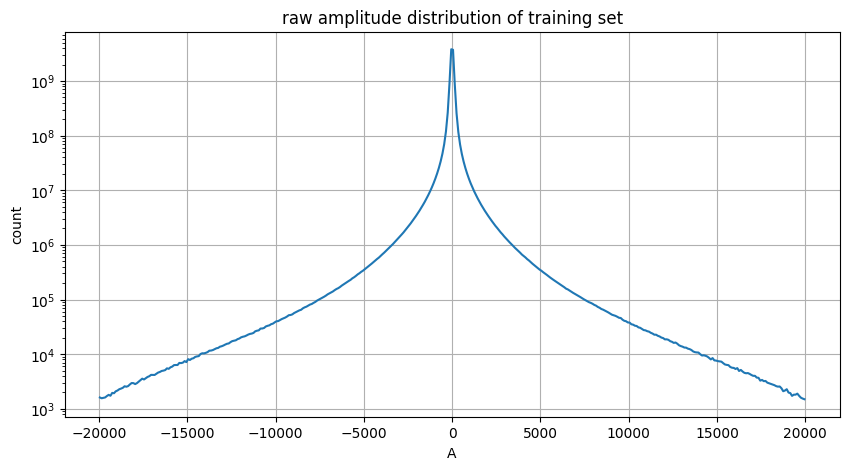
\includegraphics[width=0.55\linewidth]{unnormalized.png}
    \caption{Distribution of the raw DAS amplitudes before normalization.}
    \label{fig:raw_amplitude_distribution}
\end{figure}
This distribution makes simple linear normalization inconvenient. If the
largest amplitudes determine the scaling range, most values close to zero
are compressed into a very small interval. Alternatively, clipping the
tails would discard information contained in large-amplitude events.
The required scaling function should therefore satisfy several
properties. It should preserve the sign of the signal, remain
approximately linear around zero, compress large amplitudes, be smooth
and invertible, and avoid explicit clipping.
For this purpose, an inverse hyperbolic sine transformation is used.

\subsection{Inverse Hyperbolic Sine Transformation}

The normalized value \(y\) is computed from the raw DAS amplitude \(x\)
according to
\begin{equation}
    y
    =
    \frac{
        \operatorname{asinh}(x/s)
    }{
        \operatorname{asinh}(A_{\max}/s)
    }.
\end{equation}
The parameter \(s\) controls the transition between the approximately
linear and compressive parts of the transformation, while \(A_{\max}\)
defines the reference amplitude used for the overall normalization.
Both parameters were selected from the amplitude distribution of the
training data. The compression scale was set to \(\boldsymbol{s=50}\), which corresponds to the median absolute amplitude \(|x|\). This places the transition scale close to a typical amplitude value in the dataset, so that small amplitudes are still represented with sufficient resolution while larger values are increasingly compressed.
The reference amplitude was chosen as \(\boldsymbol{A_{\max}=12350}\), corresponding to the \(99.99\)the percentile of \(|x|\) in the training data. Using a high percentile instead of the absolute maximum prevents a very small number of extreme values from determining the normalization range. With this formulation, an amplitude equal to \(A_{\max}\) is mapped to \(\boldsymbol{y=1}\), while larger values are still represented and are not explicitly clipped.
The inverse hyperbolic sine is defined as
\(\operatorname{asinh}(z)=\ln\left(z+\sqrt{z^2+1}\right)\).
For values close to zero, \(\operatorname{asinh}(z)\approx z\), so small amplitudes are transformed approximately linearly. For larger absolute values, the function grows more slowly, which compresses the long tails of the amplitude distribution. Furthermore, \(\operatorname{asinh}(-z)=-\operatorname{asinh}(z)\), so the sign symmetry of the DAS amplitudes is preserved.
Since the transformation is invertible, the normalized values can be
mapped back to the original DAS amplitude domain after model inference.
Solving the normalization equation for \(x\) gives
\begin{equation}
    x =
    s\,
    \sinh
    \left(
        y\,
        \operatorname{asinh}(A_{\max}/s)
    \right).
\end{equation}
The transformation therefore compresses rare high-amplitude values
during training without clipping them, while still allowing the original
amplitude scale to be recovered afterwards.

\section{Inpainting and Generative Priors}

Inpainting refers to the reconstruction of missing or intentionally
removed parts of a signal using the surrounding known information. In
this thesis, traffic-related regions of a DAS patch are treated as the
regions that have to be reconstructed.
Let \(m \in \{0,1\}^{H \times W}\) denote a binary mask. The mask is
defined such that
\[
m_{ij}
=
\begin{cases}
    1, & \text{if the observation is known},\\
    0, & \text{if the position is reconstructed}.
\end{cases}
\]
If \(x\) denotes the observed DAS patch and \(\hat{x}\) denotes a
generated reconstruction, the two regions can be combined according to
\(\boldsymbol{x_{\mathrm{out}} = m \odot x + (1-m)\odot\hat{x}}\),
where \(\odot\) denotes element-wise multiplication.
This formulation ensures that the known part of the original
measurement is preserved, while only the masked region is replaced by
generated content.

For this task, the diffusion model acts as a generative prior. A
generative prior describes which signals are plausible according to the
distribution learned from the training data. Since the diffusion models
in this work are trained on traffic-free DAS data, the learned
distribution represents background-noise and earthquake-containing
signals without traffic disturbances.
During inpainting, this prior can therefore be used to generate plausible
traffic-free content for regions in which the original traffic signal has
been masked.

\chapter{Related Methods}

\section{Spatial Self-Attention}

\section{Spatial Perception and Channel Information Interaction}

\section{Mamba and Selective State-Space Models}

\section{Denoising Diffusion Implicit Models}

\section{RePaint for Diffusion-Based Inpainting}

\section{Region-Aware Diffusion}


\chapter{Diffusion-Based Inpainting of DAS Data}

\section{Denoising Architectures}

\subsection{Baseline U-Net}

\subsection{U-Net with Spatial Self-Attention}

\subsection{U-Net with SPCII}

\subsection{U-Net with Mamba}

\section{Training Objectives}

\subsection{Standard Mean Squared Error}

\subsection{Region-Weighted Mean Squared Error}

\subsection{Pixel-Weighted Mean Squared Error}

\section{DDIM and RePaint Reconstruction}

\section{Region-Aware Diffusion}


\chapter{Implementation and Experimental Setup}

\section{Dataset, Data Splits, and Data Loaders}

\section{Parameter Selection}

\subsection{Diffusion Parameters}

\subsection{Training Parameters}

\subsection{Loss Parameters}

\subsection{Sampling Parameters}

\section{Mask Selection}

\subsection{Masks for RePaint Inference}

\subsection{Masks for Region-Aware Diffusion}


\chapter{Results and Discussion}

\section{Limitations}


\chapter{Conclusion and Future Work}



% Bibliography
\bibliographystyle{ACM-Reference-Format}
\bibliography{bibliography/references}
\addcontentsline{toc}{chapter}{\bibname}

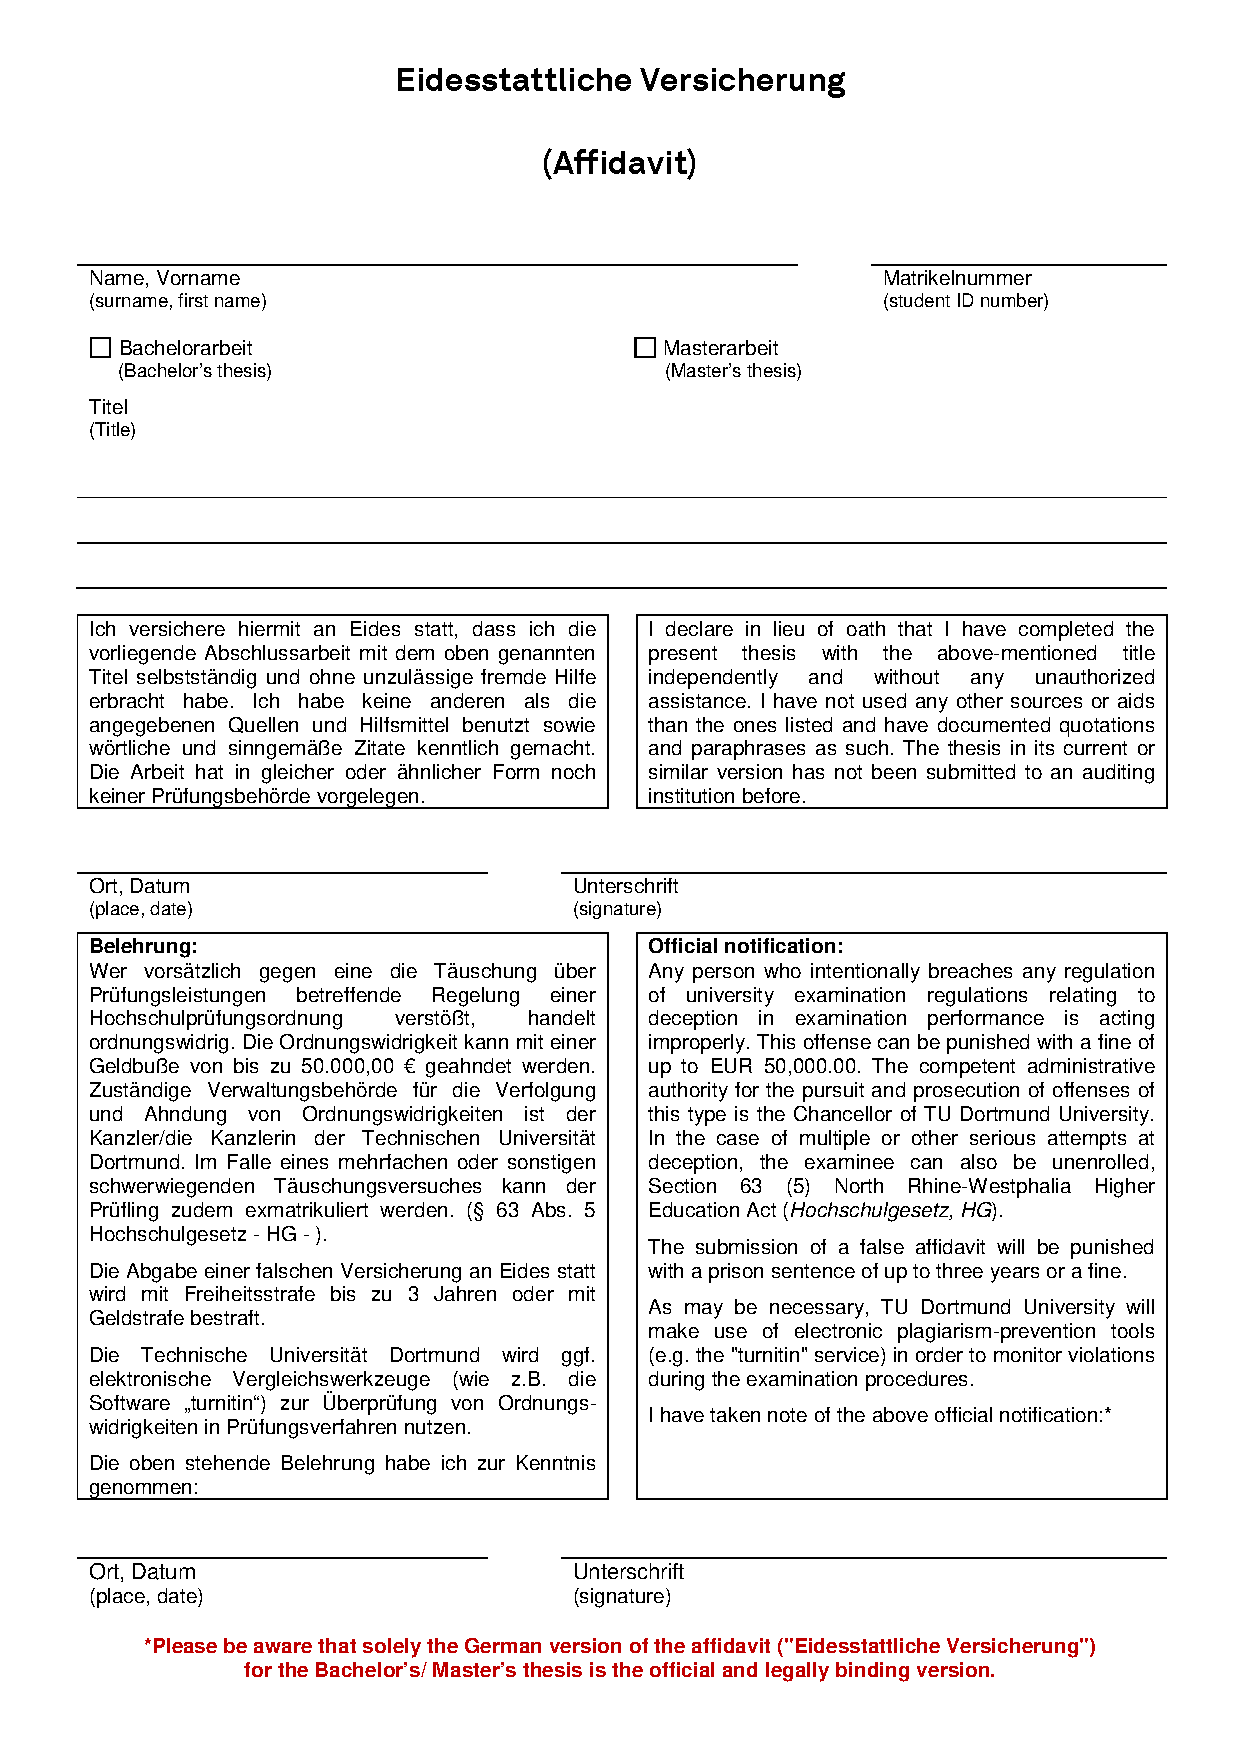
\includepdf[pages=-]{Eidesstattliche_Versicherung}

\end{document}
